\setchapterimage[6.5cm]{chapters/trees/images/trees_2.pdf}
\setchapterpreamble[u]{\margintoc}
\chapter{Trees}
\labch{trees}
In this chapter are introduced the fundamentals concepts of tree as abstract data type, and the most used algorithms related to trees \cite{wikitrees} (\href{https://en.wikipedia.org/wiki/Tree_(data_structure)}{Trees, Wikipedia}).

\section{General Definitions}
A \textbf{Tree} is an abstract datatype that simulate a hierarchical structure. A tree is a particular kind of a linked list where there are more next elements. The base element of a tree is called \textbf{Node} while the first element is called \textbf{Root}.

\begin{figure}[hb]
	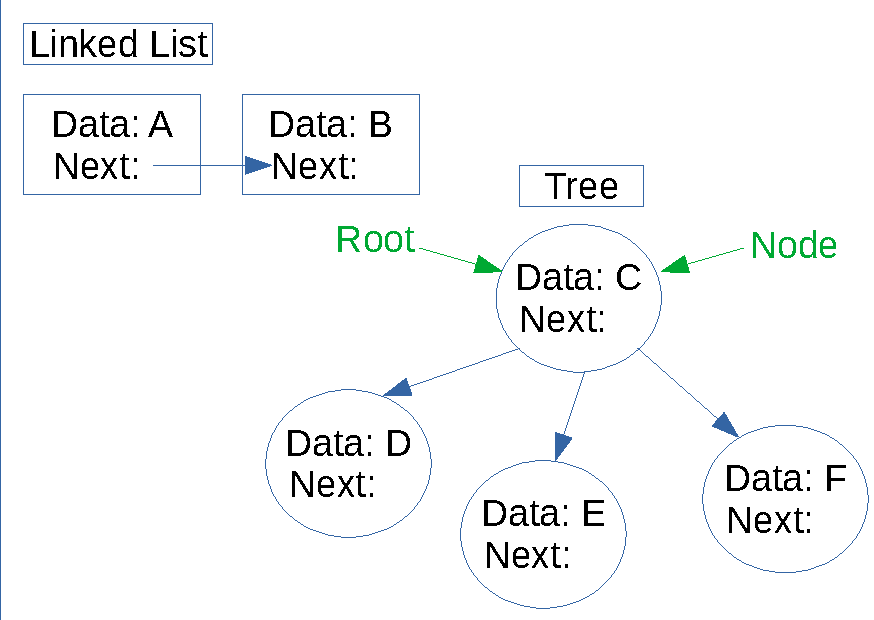
\includegraphics[width=14cm,height=6cm]{chapters/trees/images/trees_1.pdf}
	\caption[]{Elements of a tree and linked list.}
	\labfig{trees_1}
	\label{trees_1}
\end{figure}

Trees must be completed connected structures, this means that there are not any nodes which are not connected to anything (Figure \ref{trees_2} case (a)), and there must not be present any cycles (Figure \ref{trees_2} case (c)).

\begin{figure}[hb]
	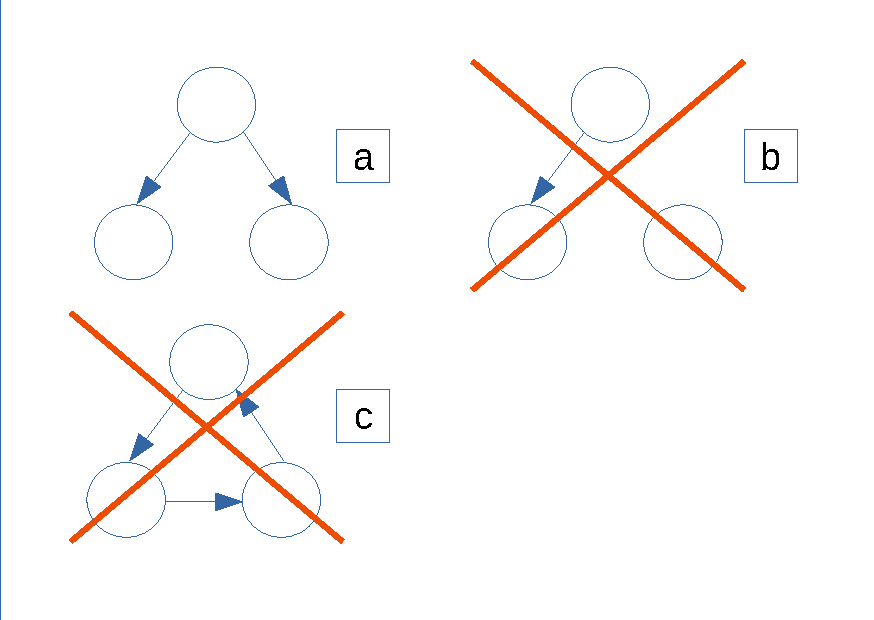
\includegraphics[width=14cm,height=6cm]{chapters/trees/images/trees_2.pdf}
	\caption[]{Completed connected structure (a), a non completed connected structure (b), and a cycle (c).}
	\labfig{trees_2}
	\label{trees_2}
\end{figure}

Trees are a hierarchical structures divided into layers: the first layer is the one belonging to the root node, the first node of a tree. The next element of the root are called children, which became parents in case they have next node connected as well. The last nodes of a trees are the nodes which do not have any children and they are called \textbf{Leaf}. The numbers of connections is called \textbf{Height}. A set of connections creates a \textbf{Path}. The numbers of edges starting from the root to a node is called \textbf{Depth}.
All this definitions are defined in following figure (Figure \ref{trees_3}).

\begin{figure}[hb]
	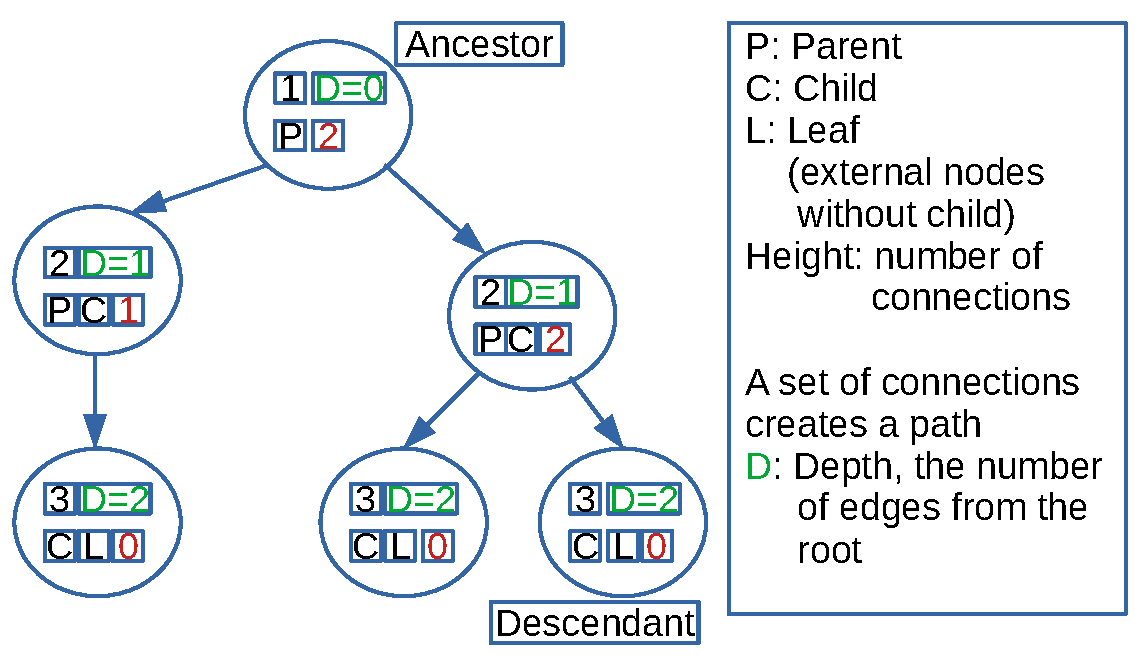
\includegraphics[width=14cm,height=6cm]{chapters/trees/images/trees_3.pdf}
	\caption[]{A tree and its fundamentals elements.}
	\labfig{trees_3}
	\label{trees_3}
\end{figure}

\section{Tree Traversal}
Which way is the most efficient for visiting all the nodes of a tree? Is it more efficient looking layer by layer or looking at subtrees?